\begin{problem}{피자 배치}{standard input}{standard output}

상언이의 단골 피자가게는 직각삼각형 모양의 테이블과 완벽한 원 모양의 피자로 유명하다. 이 가게의 사장님은 한 테이블에서 피자를 주문하면 그 테이블로 직접와서 테이블이 피자로 가득 찰 때까지 피자를 계속 만든다.

사장님은 피자 하나를 새로 만들 때 마다 다음과 같은 그만의 놀라운 방법을 사용한다. 현재 이미 만들어진 다른 피자들과 겹치지 않으면서 (접할 수는 있다) 테이블의 변 중 두개 이상에 접하도록 만들 수 있는 피자 중 가장 넓이가 큰 피자를 만든다. 상언이는 문득 이 테이블에 만들어질 $k$번째 피자의 넓이가 궁금해졌다.

\begin{center}
  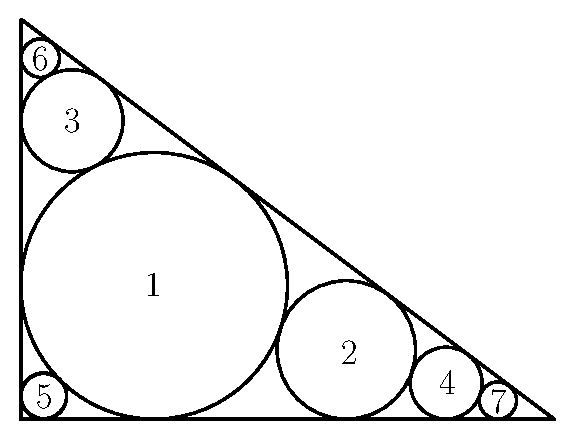
\includegraphics[width=0.8\textwidth]{pizza.eps}
\end{center}

\InputFile
첫 번째 줄에 테스트 케이스의 수 $T (1 \le T \le 10,000)$가 주어지고, 이어서 $T$개의 테스트 케이스가 입력된다.

각 테스트 케이스는 한 줄에 3개의 정수가 주어진다. 이는 직각삼각형의 직교하는 두 변 $a$, $b$의 길이와 $k$를 의미한다. ($1 \le a, b \le 10^9$, $1 \le k \le 100$)

\OutputFile
각 테스트 케이스마다, 첫 번째 줄에 $k$번째 피자의 넓이를 출력한다. 출제진의 답과 절대 오차 또는 상대 오차가 $10^{-6}$ 이하일 시 정답으로 인정한다.

\Example

\begin{example}
\exmp{1
3 4 1}{3.1415926}%
\end{example}

\end{problem}
